\chapter{Υλοποιήσεις}
\label{chapter:implementations}

Στο κεφάλαιο αυτό θα αναφερθούμε στις τρεις διαφορετικές εκδόσεις του συστήματος που
υλοποιήσαμε μέχρι να καταλήξουμε στην τωρινή και τους λόγους που μας ωθούσαν να κάνουμε αυτές τις αλλαγές.

Πριν ξεκινήσουμε όμως θα πρέπει να ορίσουμε τις βασικές ενέργειες που θα εκτελεί ένα τέτοιο σύστημα.
Αρχικά θέλουμε να έχει δυνατότητες σέρβερ, ώστε να εξυπηρετεί απομακρυσμένους χρήστες που συνδέονται μέσω του δικτύου. 
Το σύστημα επιπροσθέτως θα πρέπει να μπορεί να στέλνει αιτήματα σε εξωτερικούς σέρβερ, ιστοσελίδες και γενικά 
εφαρμογές που επικοινωνούν με το διαδίκτυο. Σε αυτό το σημείο τονίζουμε την αναγκαιότητα ύπαρξης μίας βάσης δεδομένων που θα αποθηκεύει
πληρογορία σχετική με την ορθή λειτουργία του συστήματος. Τέλος και ίσως το πιο σημαντικό, απαιτείται η ύπαρξη κάποιας
μορφής scheduling, ενός μηχανισμού δηλαδή που θα ρυθμίζει πότε θα γίνονται τα αιτήματα και ποια από αυτά πρέπει γίνουν. 

Όλα αυτά αφορούν αποκλειστικά τη λειτουργία του backend του συστήματος. Πέρα από αυτά
θα πρέπει να υπάρχει μία γραφική διεπαφή μέσω της οποίας κάθε χρήστης θα μπορεί να δει τα δεδομένα που παράγονται
από τη χρήση του συστήματός.

Πλέον και χάριν συντομίας, στο υπόλοιπο κομμάτι της διπλωματικής αυτής εργασίας, θα αναφερόμαστε
στο σύστημα που δημιουργήσαμε, με το όνομα \textbf{Lychte} (/licht/). Η ονομασία αυτή προκύπτει από τα αρχικά του "\textbf{L}ightweight
\textbf{Y}et \textbf{C}onfigurable \textbf{H}ΤTP \textbf{T}raffic \textbf{E}xpert", που περιγράφει την λειτουργία και μόνο 
μερικά από τα πολλά χαρακτηριστικά σου συστήματος μας.  

\section{Version 0.0.1}
\label{section:first_implementation}

% 1ή υλοποίηση - η πιο απλή και μη λειτουργική. Ένας node σέρβερ. Κάθε φορά που έρχεται qpi request σηκώνει καινούργιο setInterval με συγκεκριμένο interval κάθε φορά. Ιδανικό γιατί δεν θα έχεις ποτέ πρόβλημα με τον χρόνο
% 	μεταξύ διαδοχικών request επειδή είναι ακριβές. Κακή απόδοση όταν ο αριθμός των request αυξηθεί πάρα πολύ. Ξεχωριστά timer αυξάνουν την πολυπλοκότητα. Επίσης θα υπάρχει πρόβλημα όταν "πέφτει" ο σέρβερ εξαιτίας κάποιου πιθανού
%	προβλήματος. Ακόμα και να κρατάμε τα jobs σε κάποια βάση δεν θα ξέρουμε πότε πρέπει να ξανατρέξουν. Αν πχ έχεις κάποιο
%	api να τρέχει κάθε 30s και μόλις εκτελεστεί "πεσει" ο σέρβερ. Τότε θα πρέπει είτε να μην ξεκινήσεις το job και να χάσεις πιθανώς ένα request
% 	είτε να τρέξεις το job ότν και να γίνει και να έχεις διπλοεγγραφές.

Η πρώτη και πιο απλή έκδοση του υπό κατασκευής συστήματος Ενεργής Παρακολούθησης. Αποτελείται από έναν
nodejs σέρβερ (και πιο συγκεκριμένα express σέρβερ), ο οποίος είναι υπεύθυνος για τον χειρισμό όλων των λειτουργιών της εφαρμογής. Αυτός συνδέεται
άμεσα με μία MongoDB που θα αποτελέσει τη βάση δεδομένων του συστήματος.

Ο σέρβερ αρχικά στεγάζει το api της εφαρμογής. Μέσα από αυτό κάθε χρήστης που έχει πρόσβαση στο σύστημα (σωστά credentials)
μπορεί να αντλεί πληροφορία ήδη αποθηκευμένη στη βάση ή να την τροποποιεί και να δημιουργεί νέα. Τα δεδομένα που μπορεί να παράξει
είναι περιορισμένα, βέβαια, καθώς υπάρχουν collections στα οποία γράφει μόνο το backend. Για να συνεχίσουμε και να δούμε το υπόλοιπο σύστημα
θα πρεπει να αναφερθούμε στο pipeline της εφαρμογής, στα βήματα δηλαδή που θα ακολουθήσει ο χρήστης εντός αυτής.

Κύρια λειτουργία του Lychte είναι η αυτόματη παρακολούθηση του χρόνου λειτουργίας και απόκρισης ενός ιστοτόπου.
Για να γίνει αυτό ο χρήστης θα πρέπει να εισάγει το url, που επιθυμεί να επιβλέπει και να ενημερώνεται σχετικά με
τη κατάστασή του, και ένα χρονικό διάστημα βάσει του οποίου θα γίνονται επαναλαμβανόμενα αιτήματα.
Έπειτα η πληροφορία αυτή μεταφέρεται στον σέρβερ υπό τη μορφή HTTP request. Αυτός το μήνυμα που περιέχει το url και
όποια ακόμα πληροφορία απαιτείται (headers, body) για να μπορέσει να κάνει την κλήση στο εξωτερικό σύστημα
που ο χρήστης ορίζει. Τέλος αποθηκεύει το αίτημα στη βάση δεδομένων και ξεκινάει έναν απλό scheduler
ο οποίος επαναλαμβάνει το αίτημα στο url που ορίστηκε από το χρήστη ανάλογα με τον διάστημα
που επιλέχθηκε.

Καταλήγουμε έτσι στη δεύτερη, μεγάλη, λειτουργία του σέρβερ, το scheduling. Κάθε φορά που αποθηκεύεται ένα καινούργιο
αίτημα για παρακολούθηση, ξεκινάει μία νέα διεργασία εντός αυτής που ήδη τρέχει (αυτής του σέρβερ). Η διεργασία παιδί (child process),
λαμβάνει κάποια πληροφορία σχετικά με το αίτημα που θα πρέπει να εκτελεί, από την διεργασία που την δημιούργησε. Η τελευταία μάλιστα
έχει τη δυνατότητα να σταματήσει τη λειτουργία όσων διεργασιών έχει ξεκινήσει αρκεί να γνωρίζει το pid που χαρακτηρίζει κάθε μία μονοσήμαντα.

\begin{figure}[!ht]
	\centering
	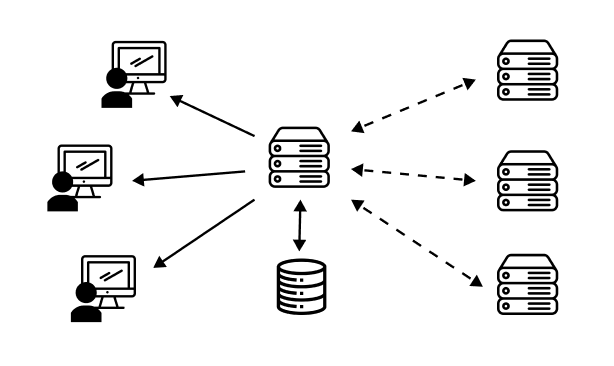
\includegraphics[width=0.8\textwidth]{./images/chapter4/lychte-first-implementation.png}
	\caption[Διάγραμμα πρώτης Υλοποίησης]{Διάγραμμα Πρώτης Υλοποίησης Συστήματος Ενεργής Παρακολούθησης. Ένας express σέρβερ, με μία mongo βάση δεδομένων εξυπηρετούν χρήστες, ενώ παράλληλα στέλνουν αιτήματα σε εξωτερικά συστήματα προς παρακολούθηση}
	\label{fig:first_implementation}
\end{figure}

Όλες οι διεργασίες εκτελούν την ίδια συνάρτηση τα ορίσματα της οποίας αποτελούν τα χαρακτηριστικά που ορίζει ο χρήστης
κατά τη διαδικασία δημιουργίας του αιτήματος προς παρακολούθηση. Η συνάρτηση αυτή είναι υπεύθυνη για να κάνει την κλήση στο εξωτερικό
σύστημα, να λάβει την απάντηση, να την αναλύσει (ανάλογα με το είδος της αναμενόμενης απάντησης) και να την αποθηκεύσει,
μαζί με κάποιες ακόμα χρήσιμες πληροφορίες, στη βάση δεδομένων. Πέρα από το response που μπορεί να είναι απλό κείμενο (html), αντικείμενο (json) ή κάποιο
αρχείο αποθηκεύονται και οι χρονισμοί του αιτήματος, το πότε δηλαδή ξεκίνησε το αίτημα, πότε τελείωσε καθώς και το χρόνο που μεσολάβησε μεταξύ τους. Το τελευταίο
θα μπορούσε να υπολογιστεί και εκ των υστέρων σε κάθε αίτημα που το χρειάζεται, καθώς είναι δεδομένο που προκύπτει από αυτά που ήδη υπάρχουν.
Εξαιτίας όμως της φύσης του συστήματος και των δεδομένων που μαζεύονται
θεωρούμε ότι κρίνεται αναγκαίο να κερδίσουμε επεξεργαστική ισχύ αποφεύγοντας υπολογισμούς 
για δεδομένα που γνωρίζουμε ότι θα ζητούνται συνεχώς, ώστε να εξηπυρετούνται όσο το δυνατό
πιο γρήγορα και άμεσα τα αιτήματα του χρήστη ως προς τον σέρβερ

Ένα τέτοιο σύστημα μπορεί να λειτουργήσει όπως ακριβώς περιγράψαμε παραπάνω. Έχει όμως κάποια βασικά μειονεκτήματα.
Αρχικά δεν υπάρχει κάποιο κοινό σημείο αναφοράς (single point of reference). Όσες διεργασίες υπάρχουν μέσα στο σέρβερ κοινούνται αυτόνομα,
χωρίς να υπάρχει κάποιος τρόπος να αναφερθείς σε κάποια αν δεν γνωρίζεις εκ των προτέρων το pid της και αν δεν έχεις πρόσβαση
στο σύστημα που τις εκτελεί. Επίσης το χαρακτηριστικό αυτό των διεργασιών έχει υπόσταση μόνο εντός του ιδίου περιβάλλοντος εκτέλεσης. Ακόμα και
να αποθηκεύαμε το pid της διεργασίας που είναι υπεύθυνο για την εκτέλεση ενός συγκεκριμένου αιτήματος, δεν θα μπορούσαμε να το χρησιμοποιήσουμε 
κάπως σε περίπτωση που επανεκκινηθεί το υπολογιστικό σύστημα που φιλοξενεί τον σέρβερ, καθώς οι καινούργιες διεργασίες θα είχαν διαφορετικό id.
Οι "καινούργιες διεργασίες" εδώ χαρακτηρίζουν ένα σύνολο διεργασιών που θα ξεκινούσε ο σέρβερ μέχρι όλα τα αιτήματα που βρίσκονται αποθηκευμένα στη βάση
να ξεκινήσουν να ελέγχονται από κάποιο process.

Αξίζει ακόμα να σημειωθεί ότι το σύστημα αυτό δεν μπορεί να κλιμακωθεί εύκολα, και αποδοτικά, καθώς 
για να επεκτείνεις το σύνολο των αιτημάτων που μπορείς να διαχειριστείς θα πρέπει να συντηρείς έναν δεύτερο σέρβερ που ίσως να μην χρειάζεται,
ώστε να χωρέσουν παραπάνω διεργασίες. Το πρόβλημα αυτό όμως μπορεί να λυθεί σπάζοντας τις δύο βασικές λειτουργίες του
Lychte σε δύο διακριτές και σαφώς ανεξάρτητες οντότητες. Ενός scheduler και ενός σέρβερ. Αυτό ακριβώς θα δούμε καινούργιες
στη δεύτερη υλοποίηση του συστήματός μας.

\newpage

\section{Version 0.1.0}
\label{section:second_implementation}

Συνεχίζοντας τη συλλογιστική πορεία της πρώτης υλοποίησης, καλούμαστε να λύσουμε ένα από τα πιο βασικά προβλήματα, που προέκυψαν
Ο διαμοιρασμός των λειτουργιών. Όπως προαναφέραμε θα πρέπει να υπάρχει ένας (ή και παραπάνω) σέρβερ που θα εξυπηρετεί
τους χρήστες μέσω διεπαφών των προγραμματιστικών διαδικασιών που παρέχει, και ένας (ή παραπάνω) scheduler, που θα εκτελούν
αποκλειστικά και μόνο αιτήματα προς τα συστήματα που θέλουμε να ελέγχουμε. Ας δούμε όμως πιο συγκεκριμένα το ανανεωμένο σύστημα (\autoref{fig:second_implementaion})

\begin{figure}[!ht]
	\centering
	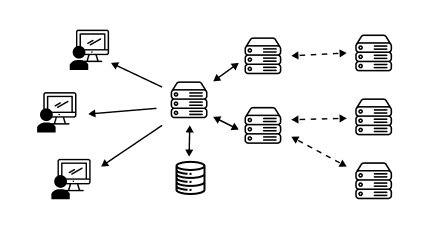
\includegraphics[width=0.8\textwidth]{./images/chapter4/lychte-second-implementation.png}
	\caption[Διάγραμμα δεύτερης Υλοποίησης]{Διάγραμμα Δεύτερης Υλοποίησης Συστήματος Ενεργής Παρακολούθησης. Αποτελείται στο κέντρο του από έναν express σέρβερ και μία mongo βάση δεδομένων. Ο σέρβερ επικοινωνεί με δύο schedulers οι οποίοι είναι υπεύθυνοι για τον έλεγχο εξωτερικών προς το σύστημα εφαρμογών/σέρβερ}
	\label{fig:second_implementaion}
\end{figure}

Το βασικό συστατικό του Lychte, ο σέρβερ δηλαδή παραμένει όπως είχε. Έχει δηλαδή routes μέσα από τα οποία εξυπηρετεί αιτήματα
των χρηστών που προέρχονται από το frontend του συστήματος. Αυτά αφορούν την αποστολή πληροφορίας προς τους χρήστες προκειμένου να δουν
τα δεδομένα που αποθηκεύουμε στη βάση μας, αλλά και την αποθήκευση πληροφορίας που προέρχεται από τους χρήστες που σχετίζεται με τη δημιουργία
καινούργιων ελέγχων σε urls που επιθυμούν να παρακολουθούν.

Αυτό που αλλάζει σε σχέση με την προηγούμενη υλοποίηση, είναι ο τρόπος που διευθετεί
την εκτέλεση των επαναλαμβανόμενων αιτημάτων που πρέπει να κάνει προς τα εξωτερικά υπό παρακολούθηση συστήματα.
Όπως είπαμε νωρίτερα δεν είναι πλέον υπεύθυνος για το scheduling των ενεργειών που πρέπει να γίνουν, 
αλλά αντιθέτως στέλνει σε ένα άλλο σύστημα (scheduler) τις πληροφορίες που χρειάζεται προκειμένου να ρυθμιστεί και να οργανωθεί κατάλληλα
 ο έλεγχος των urls που θέλουμε να ελέγχονται.

Πλέον θα αναφερόμαστε στο σύστημα του scheduler ως worker, καθώς αυτό που κάνει είναι να λαμβάνει δεδομένα και να
εκτελεί βάση αυτών συνεχώς αιτήματα προς άλλα εξωτερικά συστήματα. Ο τρόπος λειτουργίας του είναι αρκετά παρόμοιος
με τη αυτή του scheduler της πρώτης υλοποίησης, με κάποιες μικρές διαφορές. Κάθε φορά που λαμβάνει κάποιο αίτημα από τον κεντρικό σέρβερ, κάνει ένα δοκιμαστικό request
στο url που πρόκειται να ελεγχθεί, για να διαπιστωθεί η ορθότητά του. Έπειτα ξεκινάει έναν timer που εκτελεί το αίτημα ανά
χρονικό διάστημα που ορίζει ο χρήστης. Ο χρόνος αυτός μπορεί να φτάνει ένα κάτω όριο του ενός δευτερολέπτου, αλλά για λόγους σταθερότητας και
εγγύησης ότι η εκτέλεση κάποιου αιτήματος δεν θα μπλοκάρει την εκτέλεση κάποιου άλλου, έχουμε βάλει ένα κάτω όριο των 30 δευτερολέπτων στην υλοποίησή μας.
Στην περίπτωση που το αίτημα χρειαστεί χρόνο, για να ικανοποιηθεί, μεγαλύτερο αυτού που έχει οριστεί σαν χρόνος μεταξύ
διαδοχικών αιτημάτων διακόπτουμε το αίτημα μέσω timeouts και το αποθηκεύουμε στη βάση σαν αποτυχημένη απόκριση (failed response).
Αυτό γίνεται για να εξασφαλίσουμε ότι το χρονικό διάστημα μεταξύ διαδοχικών αιτημάτων θα παραμένει
σχετικά σταθερό και η απόλυτη μετατόπιση του χρόνου που υπάρχει μεταξύ των αιτημάτων σε βάθος χρόνου. 
δεν θα αλλάζει σε μεγάλο βαθμό.

Για να γίνει πιο κατανοητό το παραπάνω αρκεί να μελετήσουμε τα \autoref{fig:perfect_request_cycle} και \autoref{fig:timeouts_request_cycle}

Το πρώτο περιγράφει την εκτέλεση ενός αιτήματος ανά ένα χρονικό διάστημα ενός λεπτού. Όπως παρατηρούμε το
αίτημα εκτελείται σε αυτό το μήκος χρόνου με αποτέλεσμα, όταν ξαναέρθει η στιγμή που πρέπει να επαναεκτελεστεί,
αυτό να γίνει χωρίς περιττές καθυστερήσεις. Αν υποθέσουμε ότι ο χρόνος που μεσολάβησε μεταξύ του πρώτου και του δεύτερου αιτήματος
είναι ακριβώς εξήντα δευτερόλεπτα μπορούμε να πούμε ότι η απόκλιση, σε σχέση με τον ένα λεπτό, μεταξύ των αυτών είναι μηδενική.
Βέβαια κάτι τέτοιο δεν υφίσταται στην πραγματικότητα καθώς οι timers έχουν πάντα μία μικρή απόκλιση, προς τα πάνω ή προς τα κάτω, της τάξης των nanoseconds.
Σε βάθος χρόνου η απόκλιση παραμένει κοντά στο μηδέν.

\begin{figure}[!ht]
	\centering
	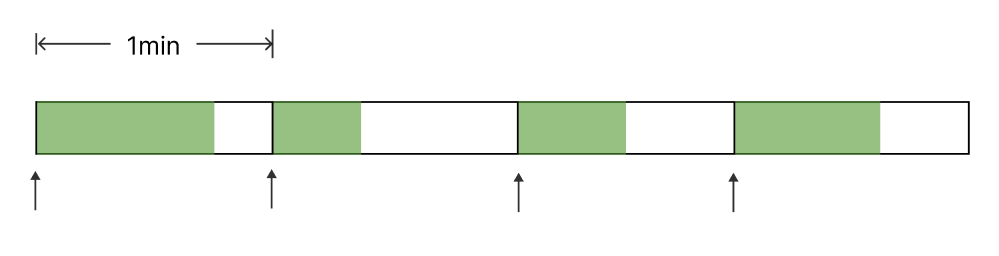
\includegraphics[width=0.8\textwidth]{./images/chapter4/perfect_request_cycle.png}
	\caption[Κύκλος Ζωής εκτέλεσης ενός επαναλαμβανόμενου Αιτήματος]{Κύκλος Ζωής εκτέλεσης ενός επαναλαμβανόμενου Αιτήματος}
	\label{fig:perfect_request_cycle}
\end{figure}

Έπειτα ας μελετήσουμε την περίπτωση που το αίτημα χρειάζεται παραπάνω χρόνο για να εκτελεστεί (εξαιτίας καθυστερήσεων του εξωτερικού συστήματος που ελέγχεται).
Στο \autoref{fig:timeouts_request_cycle} μπορούμε να δούμε ακριβώς πως θα λειτουργούσε ένας worker στην περίπτωση που υπήρχαν μεγάλες εξωγενείς καθυστερήσεις, χωρίς τη χρήση
timeous αλλά και με τη χρήση αυτών. Όταν αναφερόμαστε σε timeouts περιγράφουμε την πρόωρη έξοδο από τη συνάρτηση που τρέχουμε, στην
προκειμένη, η εκτέλεση του αιτήματος. Παρατηρούμε ότι στα δύο χρονικά διαγράμματα έχουμε αρκετά μεγάλες διαφορές.
Στο πρώτο περιμένουμε να εκτελεστεί πλήρως το αίτημα, ακόμα και αν αυτό αργήσει παραπάνω από όσο
θα έπρεπε. Το επόμενο αίτημα ξεκινάει με κάποια καθυστέρηση ως προς το πρώτο και παρομοίος τα επόμενα στη σειρά.
Αυτή η διαδικασία εισάγει απόκλιση στους χρόνους των κλήσεων μεταξύ των αιτημάτων που υπό φυσιολογικές συνθήκες αναμένουμε να ισαπέχουν (χρονικά) μεταξύ τους.
Απόκλιση η οποία μάλιστα μπορεί συνεχώς να αυξάνεται, καθιστώντας το σύστημά μας αναξιόπιστο ως προς
το χρόνο εκτέλεσης και την ακρίβεια των αιτημάτων. Για αυτό το λόγο κρίνουμε αναγκαία τη χρήση timeouts.
Το μεινέκτημα σε αυτή την περίπτωση είναι ότι αποθηκεύουμε ως εσφαλμένο ένα πιθανώς σωστό response, λόγω του χρόνου που πήρε για να εκτελεστεί.

\begin{figure}[!ht]
	\centering
	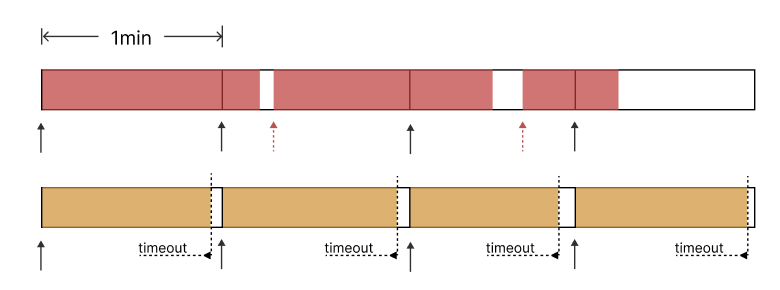
\includegraphics[width=0.8\textwidth]{./images/chapter4/timeout_request_cycle.png}
	\caption[Σύγκριση χρήσης ή μη timeouts στον κύκλο ζωής εκτέλεσης ενός αργού επαναλαμβανόμενου αιτήματος]{Σύγκριση χρήσης ή μη timeouts στον κύκλο ζωής εκτέλεσης ενός αργού επαναλαμβανόμενου αιτήματος}
	\label{fig:timeouts_request_cycle}
\end{figure}

Μία ακόμα αλλαγή ως προς την πρώτη υλοποίηση αφορά την επικοινωνία μεταξύ σέρβερ και worker. Προκειμένου το σύστημα να
μπορεί να σπάσει σε πιο διακριτές έννοιες χάνουμε το πλεονέκτημα του να έχουμε όλες τις λειτουργίες εντός του ίδιου συστήματος.
Λειτουργίες οι οποίες πλέον για να επιτελούνται πρέπει να υπάρχει ένα τρόπος επικοινωνίας μεταξύ των εμπλεκόμενων.
Η επικοινωνία αυτή δεν θα είναι απαραίτητα μονόπλευρη. Η βασική λειτουργία όπως είχαμε δει και από την προηγούμενη υλοποίηση
είναι η αποστολή μηνυμάτων στον scheduler, σε αυτή την περίπτωση στον worker. Επεκτείνοντας όμως τις δυνατότητες του συστήματος
θα μπορούσαμε να έχουμε αμφίδρομη επικοινωνία μεταξύ σέρβερ και worker, ώστε να μπορεί να ενημερώνεται ο σέρβερ (όταν το ζητήσει) για την
κατάσταση των διαφόρων worker που είναι συνδεμένοι σε αυτόν. Κάτι τέτοιο θα είχε νόημα αν είχαμε παραπάνω από έναν worker και θα θέλαμε να κάνουμε
διαμοιρασμό φόρτου σε καθέναν από αυτούς. Αρχικά θα ρωτούσε όλους τους συνδεδεμένους worker σχετικά με το πλήθος των αιτημάτων
που ελέγχουν τη δεδομένη χρονική στιγμή. Έπειτα κάθε κόμβος θα απαντούσε και αυτός με το λιγότερο φόρτο θα επιλεγόταν ως ο κατάλληλος 
για τη δημιουργία μίας ακόμα διεργασίας ελέγχου ενός url.

Λόγω της αμφίδρομης σχέσης που έχουν τα δύο συστήματα μεταξύ τους, επιλέχθηκε το πρωτόκολλο επικοινωνίας των WebSockets.
Πιο συγκεκριμένα ο τρόπος ενσωμάτωσης της τεχνολογίας αυτής πραγματοποιήθηκε με τη χρήση της βιβλιοθήκης socket.io που αποτελεί ένα
abstract layer πάνω από το πρωτόκολλο WebSockets. Για να υπάρξει επικοινωνία θα πρέπει να υπάρχει από τη μία πλευρά ένας \textbf{socket.io-server} και από την άλλη, ένας \textbf{socket.io-client}.
Στη δική μας εφαρμογή ο socket.io-server θα είναι ο σέρβερ και ο socket.io-client ο worker. Κάθε φορά που θα ξεκινάει τη λειτουργία του ένας σέρβερ θα δημιουργεί στο τοπικό δίκτυο του
έναν socket server στον οποίο μπορούν να συνδεθούν και να επικοινωνήσουν όσοι διαθέτουν το url και τα απαραίτητα credentials. Από την άλλη
κάθε φορά που ξεκινάει τη λειτουργία του ένας worker θα πρέπει να μπορεί να συνδέεται κατευθείαν στο socket server που υπάρχει.
Θα πρέπει δηλαδή να διαθέτει από πριν το url που οδηγεί στον socket server του σέρβερ.

Οι λόγοι που επιλέχθηκαν τα WebSockets αντί ενός κλασσικού HTTP σέρβερ είναι κυρίως η ταχύτητα που προσφέρουν. Υπό περιτπώσεις
μπορεί να είναι μέχρι και δέκα φορές πιο γρήγορα σε σχέση με το συμβατικό πρωτόκολλο HTTP. Επίσης από τη στιγμή που κάθε worker 
θα επικοινωνεί αποκλειστικά με έναν (ή περισσότερους) βλέπουμε ότι δεν έχει νόημα η δημιουργία ολόκληρου σέρβερ στο πλαίσιο ενός worker.

\begin{figure}[!ht]
	\centering
	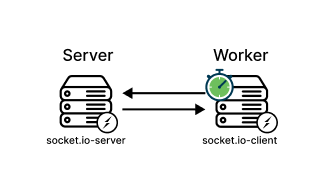
\includegraphics[width=0.8\textwidth]{./images/chapter4/socket.io-communication.png}
	\caption[Επικοινωνία σέρβερ-worker μέσω websockets]{Επικοινωνία σέρβερ-worker μέσω websockets}
	\label{fig:socketio-communitation}
\end{figure}

Η παραπάνω υλοποίηση έχει πολλά πλεονεκτήματα σε σχέση με την πρώτη. Αρχικά με τον καταμερισμό
των δύο βασικών λειτουργιών κερδίζουμε όσων αφορά την πολυπλοκότητα του συστήματος, κάτι το οποίο θα πρέπει να μας απασχολεί,
καθώς όσο πιο πολύπλοκο είναι ένα σύστημα τόσο πιο δύσκολα συντηρείται στη συνέχεια. Πέρα από αυτό, που αφορά
κυρίως τη διαδικασία ανάπτυξης λογισμικού και δεν επιφέρει κάποιο άμεσο κέρδος στους χρήστες, θα πρέπει να αναφέρουμε
ότι το σύστημα γενικά είναι πιο αποδοτικό, καθώς οι διεργασίες που κάθε worker στεγάζει είναι λιγότερο πιθανό να
κολλήσουν και να μπλοκάρουν λόγω φόρτου στο μηχάνημα που εκτελούνται. Τα requests γενικά δεν καταναλώνουν πολλούς πόρους από το σύστημα στο οποίο εκτελούνται,
σε αντίθεση με έναν server που μπορεί να δέχεται συνεχώς αιτήματα. Αξίζει να σημειωθεί ότι το api που παρέχει ο server είναι υπεύθυνο
για την αποστολή μεγάλου πλήθος πληροφορίας συνεχώς, που χρησιμοποιείται σε πληθώρα διαγραμμάτων, καθιστώντας τον έτσι απαιτητικό ως προς τους πόρους του
συστήματος. 

Ένας ακόμα τομέας στον οποίο συνεισφέρει σε μεγάλο βαθμό η διάσπαση των λειτουργιών αφορά την κλιμάκωση, και βασικά την οριζόντιο κλιμάκωση
του συστήματος. Αν δούμε ότι ο σέρβερ υστερεί και δυσκολεύεται να ανταπεξέλθει στα αιτήματα των χρηστών,
μπορούμε να φτιάξουμε έναν καινούργιο σέρβερ. Από την άλλη, αν παρατηρήσουμε ότι οι worker αργούν ή έχουν υπερφορτωθεί
μπορούμε να δημιουργήσουμε workers.

Ακόμα και με αυτή την υλοποίηση υπάρχει έλλειψη ενός κοινού σημείου αναφοράς. Ενός κόμβου στο σύστημά μας του οποίου
οι αλλαγές θα επηρέαζαν άμεσα τη λειτουργία όλων των οντοτήτων αυτού.  